\begin{figure*}[!h]
    \centering
    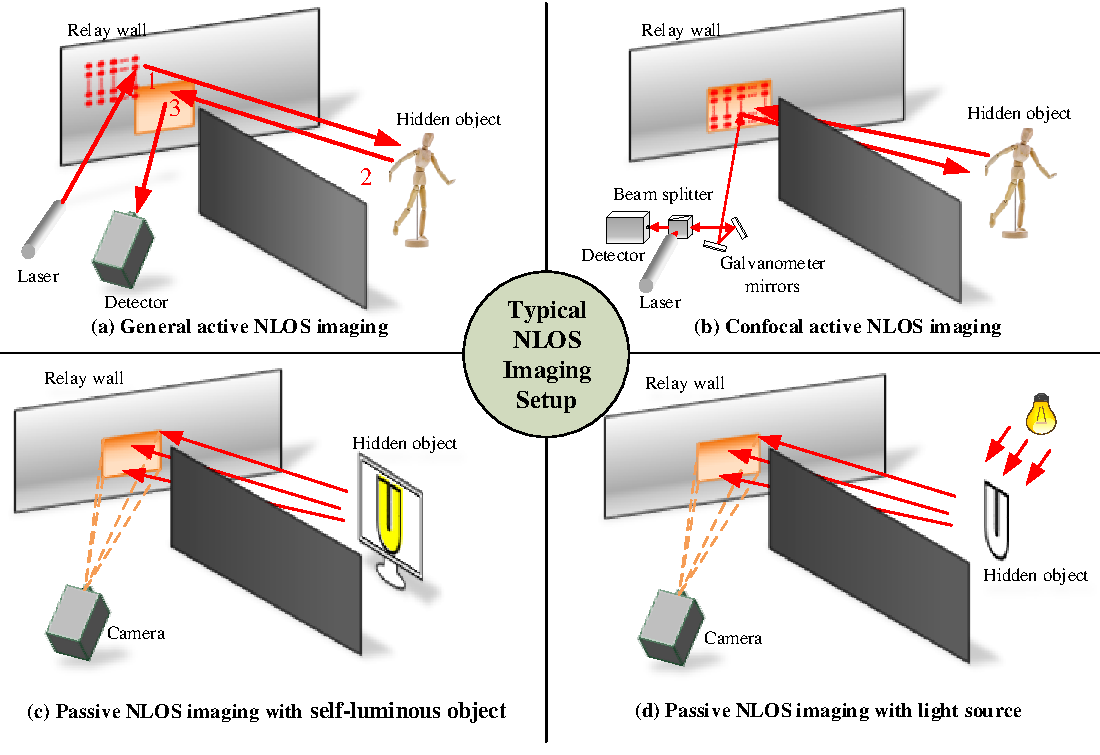
\includegraphics[width=1\textwidth]{./pic/Fig1_overview.pdf}
    \caption{Four typical NLOS imaging setups}
    \label{fig:introFig}
\end{figure*}

\section{Introduction}
\bookmark[dest=\HyperLocalCurrentHref,level=1]{Introduction}
With the rapid development of photon-sensitive sensors and imaging algorithms, optical imaging capabilities have been greatly improved in recent years. Within the line of sight, high-quality imaging can be achieved at a relatively long distance. However, due to the inherent physical constraint of visible light, traditional optical imaging is difficult to see objects outside the line of sight. To break that restriction, non-line-of-sight(NLOS) imaging analyzes the diffuse reflection from a relay wall to image hidden objects, which has broad applications in many fields, such as medical imaging, autonomous driving, and robotic vision~\cite{otooleConfocalNonlineofsightImaging2018,liuVirtualWaveOptics2018}.

According to whether a controllable light source is used, NLOS imaging can be divided into active imaging and passive imaging. Active NLOS imaging often uses expensive external light sources with high temporal resolution(e.g., ultrafast laser) to illuminate the diffuse relay surface. Simultaneously, a sensitive time-resolved detector is used to detect the light reflected on the relay surface, hidden objects, and relay surface in sequence.
The collected effective light is often referred as the three-bounce light since it is reflected by three surfaces (relay surface, hidden objects, and relay surface) in succession. 
Then, the collected three-bounce light is analyzed by different algorithms(e.g., backprojection\cite{veltenRecoveringThreedimensionalShape2012,arellanoFastBackprojectionNonline2017}, inverse methods\cite{heideDiffuseMirrors3D2014} and wave-based methods\cite{liuPhasorFieldDiffraction2020,Lindell:2019:Wave}) to reconstruct the hidden scene.
Since the active methods can collect different kinds of information, including intensity, time, and coherence, the active methods can perform a high-resolution 3D reconstruction. On the other hand, passive methods do not use a controllable external light source but use ambient light or light emitted by hidden objects to complete NLOS imaging. Despite the low cost, passive methods usually can only collect intensity\cite{saundersComputationalPeriscopyOrdinary2019} or limited coherence information\cite{batarsehPassiveSensingCorner2018a,boger-lombardPassiveOpticalTimeofflight2019} and usually complete low-quality 2D reconstruction or localization, while a few recent works can estimate hidden scene position or depth with partial occluders~\cite{saundersComputationalPeriscopyOrdinary2019,seidelTwoDimensionalNonLineofSightScene2020}.

\begin{figure*}[!h]
    \centering
    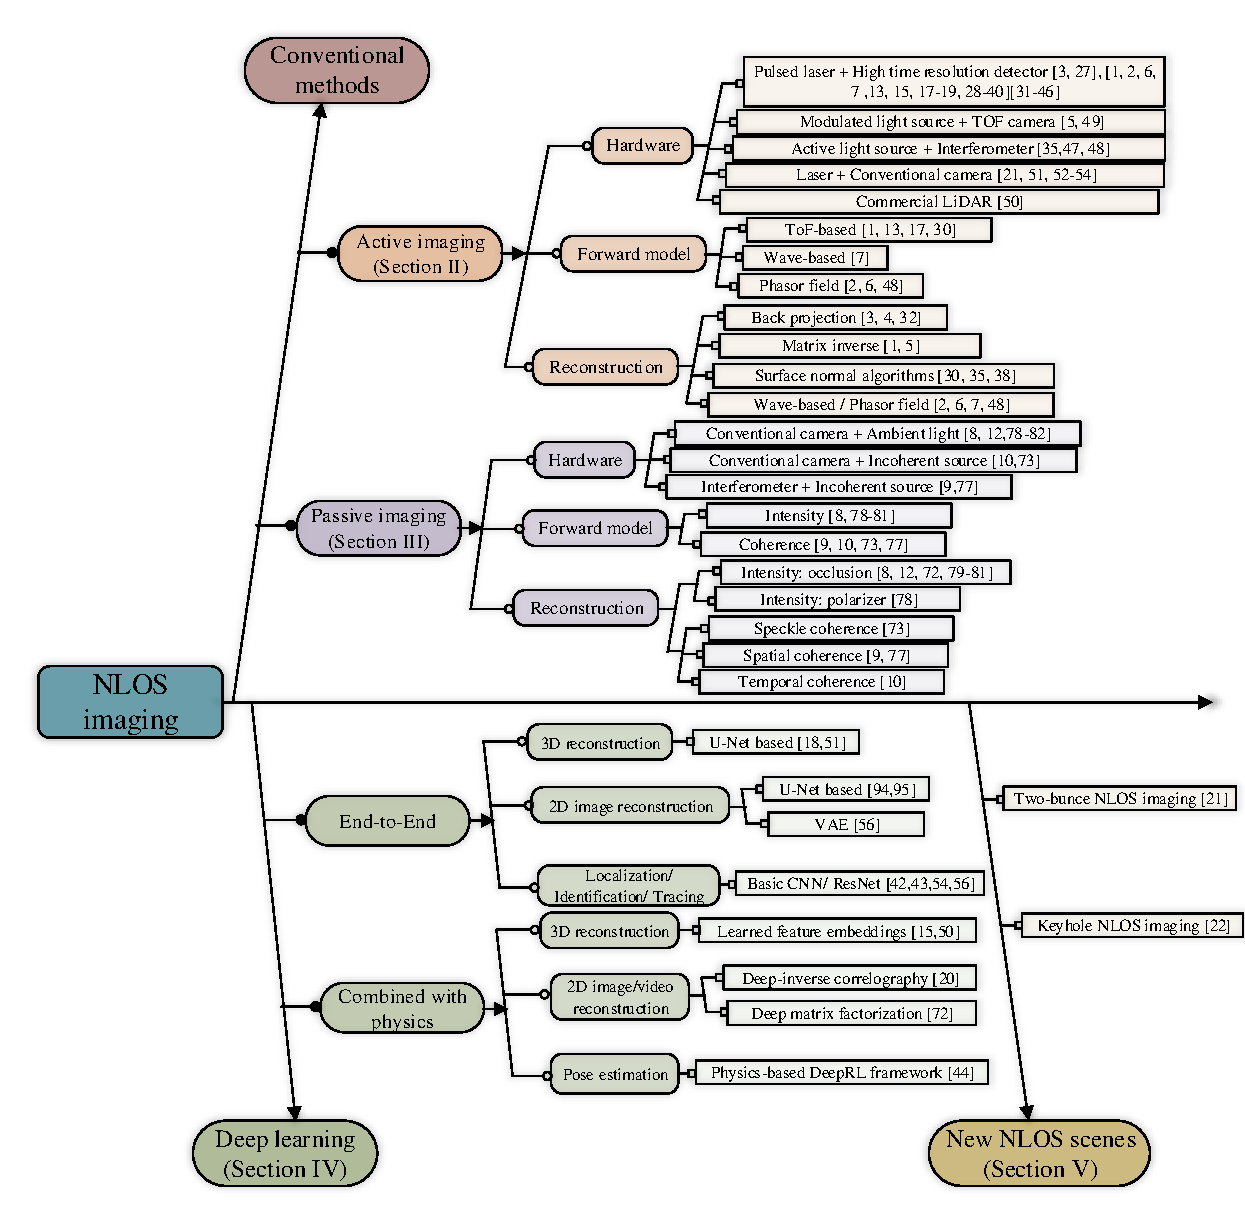
\includegraphics[width=1\textwidth]{./pic/Fig2_overview_tree.pdf}
    \caption{An overview of NLOS imaging.}
    \label{fig:introTree}
\end{figure*}

Four typical NLOS imaging setups are shown in Figure~\ref{fig:introFig}, and there are many challenges when realizing the NLOS imaging. First, due to the high-order loss with distance and environmental noise during the light transport process, NLOS imaging is an ill-posed problem with low SNR, making high-quality reconstruction extremely difficult~\cite{thrampoulidisExploitingOcclusionNonLineofSight2018}. Different hidden scenes may produce the same measurement, which deepens the ill-posedness of the problem~\cite{liuAnalysisFeatureVisibility2019}. Second, the spatial resolution of the reconstruction result is limited by the size of the scanning area (aperture size) and the system's temporal resolution. When the size of the hidden scene is large or complex, the spatial resolution will be limited by the computational complexity~\cite{otooleConfocalNonlineofsightImaging2018}. Third, the data collection time is too long~\cite{yeCompressedSensingActive2021}. Typical time-resolved NLOS imaging needs a scanning process to obtain data, making it difficult to reconstruct in real-time with high quality. Although array detectors (e.g., SPAD array) are promising to eliminate the scanning process~\cite{jinScannerlessNonlineofsightThree2020}, they have not yet been fully explored.


Despite the difficulties, many emerging innovative methods have achieved NLOS imaging under certain scenarios in recent years.
Figure \ref{fig:introTree} summarizes recent NLOS imaging research.
It can be seen that the conventional methods based on physical imaging models, are still the mainstream of research in recent years.
Conventional methods rely on imaging setup and illumination (e.g., active or passive), which are committed to developing three factors in NLOS imaging: advanced hardware systems, accurate forward imaging models and effective reconstruction algorithms. 
For example, \cite{wuNonLineofsightImaging2021} deployed confocal settings and dual-telescope to complete an amazing 1.43km NLOS imaging. Liu \etal exploited the phasor field to convert NLOS imaging model to LOS imaging model\cite{liuVirtualWaveOptics2018,liuPhasorFieldDiffraction2020}, thus achieving high-quality reconstruction of complex scenes. \cite{otooleConfocalNonlineofsightImaging2018} subtly converted NLOS reconstruction into a three-dimensional deconvolution problem. All these works have greatly promoted the development of NLOS imaging.

Besides conventional methods, the application of deep learning in NLOS imaging has also been rapidly developed. According to network design principles, the deep learning methods used in NLOS imaging are divided into end-to-end networks\cite{chopiteDeepNonLineofSightReconstruction2020} and physics-based networks\cite{chen_learned_2020,metzlerDeepinverseCorrelographyRealtime2020}. Compared with conventional algorithms, deep learning algorithms can thoroughly learn the scene prior, automatically extract features, and complete the reconstruction of hidden objects. Although NLOS imaging based on deep learning is still at the early stage, it has broad research prospects for practical applications.
Moreover, some new types of NLOS scenes, such as “imaging behind occluders” \cite{vedaldi_imaging_2020} that used two reflections behind obstacles and keyhole imaging\cite{metzler_keyhole_2021}, have also been proposed, enriching the applications of NLOS imaging. This article aims to make a detailed review of the various types of NLOS imaging research mentioned above, including conventional active and passive methods, deep learning-based NLOS imaging, and new NLOS scenarios. The corresponding challenges and opportunities will also be discussed. We hope this article can help readers have a systematic understanding of existing NLOS imaging research.

Compared to the existing surveys\cite{maedaRecentAdvancesImaging2019,faccioNonlineofsightImaging2020}, this article is much more comprehensive with the coverage of different NLOS imaging scenes, deep learning algorithms, and new NLOS imaging scenarios. As an emerging technology that has developed rapidly in recent years, the algorithms and applicable scenarios of NLOS imaging are constantly growing. Survey~\cite{maedaRecentAdvancesImaging2019} summarized the research of NLOS imaging in detail by classifying existing methods based on ToF information, coherent information, and intensity information. However, it completes the review from the perspective of the information used, and has less introduction to imaging models, reconstruction algorithms, and recent deep learning methods. Besides, in \cite{maedaRecentAdvancesImaging2019}, the passive imaging problem was only a subset of different exploited information and thus not described in detail. Another review~\cite{faccioNonlineofsightImaging2020} provided and summarized the key technologies of laser-based active NLOS imaging, which however lacked the description of passive NLOS imaging, deep learning methods and new NLOS scenes. On the contrary, this article summarizes the latest active and passive NLOS imaging research based on physical methods and provides a detailed summary and analysis of the latest deep learning algorithms, including the advantages, types, challenges, and prospects. Besides, this article also summarizes several new types of NLOS imaging scenarios. Notice that such summarization can help readers have an overall understanding of NLOS imaging, which however cannot be found in the existing surveys~\cite{maedaRecentAdvancesImaging2019, faccioNonlineofsightImaging2020}.

The remainder of this article is organized as follows. In Section \ref{sec2}, we first introduce the existing work of active NLOS imaging from three aspects: the hardware, forward propagation model, and reconstruction algorithms. We also discuss the challenges and prospects of active NLOS imaging. Then, in Section~\ref{sec3}, the related work, including the hardware, forward model, and reconstruction algorithms, as well as the challenges and prospects of passive NLOS methods, are summarized respectively. In Section ~\ref{sec4}, we review the deep learning algorithms that have emerged in recent years from their motivations, network structures, loss functions, corresponding challenges, and prospects. The new NLOS imaging scenarios are discussed in Section~\ref{sec5} and conclusions are drawn finally in Section~\ref{sec6}.
Figure~\ref{fig:introTree} clearly illustrates the relationship between the structure of this article and the current development of NLOS imaging technologies.
It should be noted that imaging through a scattering medium\cite{lindell_three-dimensional_2020,bertolotti_non-invasive_2012} does not belong to the NLOS imaging scope in this article.

\vspace{0.8mm}
\noindent \textbf{Update (2022--2026).}
Since the original version of this survey (published in 2021), NLOS imaging has undergone rapid and dramatic advances across all fronts.
On the hardware side, novel detector designs such as gradient-gated SPAD arrays~\cite{zhaoGradientGatedSPAD2023} and superconducting nanowire single-photon detectors (SNSPDs) operating at infrared wavelengths~\cite{fengSNSPD2023} have extended the capability of time-resolved systems.
On the algorithmic side, the introduction of transformer-based architectures~\cite{liNLOST2023,liTransiT2025}, state-space models~\cite{liMambaTemporalConsistency2024}, graph neural networks~\cite{suDGNLOS2025}, and diffusion model priors~\cite{suModelGuidedDiffusion2024} has significantly advanced the reconstruction quality and real-time performance of NLOS systems. Real-time NLOS video at 4\,fps for room-sized dynamic scenes has been demonstrated~\cite{yeRealTimeNLOS2024}, marking a landmark towards practical deployment. Beyond the classical optical setting, NLOS imaging has been extended to mmWave radar~\cite{laiHoloRadar2025} and ultrasound~\cite{ultrasoundNLOS2025}, opening new application domains. New NLOS scenes have also emerged, including human pose estimation~\cite{xiaoHumanPose2026} and polarization-based scanning-free single-pixel imaging~\cite{zhouPolarizationSinglePixel2026}. This updated survey incorporates these advances and provides an up-to-date reference for researchers in the field.
